\documentclass[]{article}

\usepackage{graphicx,type1cm,eso-pic,color}
\usepackage[spanish]{babel} %%%% for


\makeatletter
          \AddToShipoutPicture{
            \setlength{\@tempdimb}{.95\paperwidth}
            \setlength{\@tempdimc}{.5\paperheight}
            \setlength{\unitlength}{1pt}
            \put(\strip@pt\@tempdimb,\strip@pt\@tempdimc){
        \makebox(0,0){\rotatebox{-90}{\textcolor[gray]{0.90}
        {\fontsize{.65cm}{.5cm}\selectfont{\rm Dae-Jin Lee}}}}
            }
        }
          \AddToShipoutPicture{
            \setlength{\@tempdimb}{.50\paperwidth}
            \setlength{\@tempdimc}{.95\paperheight}
            \setlength{\unitlength}{1pt}
            \put(\strip@pt\@tempdimb,\strip@pt\@tempdimc){
        \makebox(0,0){\rotatebox{0}{\textcolor[gray]{0.90}
        {\fontsize{.5cm}{.5cm}\selectfont{\rm Curso de Estad\'istica b\'asica para Data Scientist  - @datahack}}}}
            }
        }
\makeatother

\def\tightlist{}

\usepackage{lmodern}
\usepackage{amssymb,amsmath}
\usepackage{ifxetex,ifluatex}
\usepackage{fixltx2e} % provides \textsubscript
\ifnum 0\ifxetex 1\fi\ifluatex 1\fi=0 % if pdftex
  \usepackage[T1]{fontenc}
  \usepackage[utf8]{inputenc}
\else % if luatex or xelatex
  \ifxetex
    \usepackage{mathspec}
    \usepackage{xltxtra,xunicode}
  \else
    \usepackage{fontspec}
  \fi
  \defaultfontfeatures{Mapping=tex-text,Scale=MatchLowercase}
  \newcommand{\euro}{???}
\fi
% use upquote if available, for straight quotes in verbatim environments
\IfFileExists{upquote.sty}{\usepackage{upquote}}{}
% use microtype if available
\IfFileExists{microtype.sty}{%
\usepackage{microtype}
\UseMicrotypeSet[protrusion]{basicmath} % disable protrusion for tt fonts
}{}
\usepackage{color}
\usepackage{fancyvrb}
\newcommand{\VerbBar}{|}
\newcommand{\VERB}{\Verb[commandchars=\\\{\}]}
\DefineVerbatimEnvironment{Highlighting}{Verbatim}{commandchars=\\\{\}}
% Add ',fontsize=\small' for more characters per line
\usepackage{framed}
\definecolor{shadecolor}{RGB}{248,248,248}
\newenvironment{Shaded}{\begin{snugshade}}{\end{snugshade}}
\newcommand{\KeywordTok}[1]{\textcolor[rgb]{0.13,0.29,0.53}{\textbf{{#1}}}}
\newcommand{\DataTypeTok}[1]{\textcolor[rgb]{0.13,0.29,0.53}{{#1}}}
\newcommand{\DecValTok}[1]{\textcolor[rgb]{0.00,0.00,0.81}{{#1}}}
\newcommand{\BaseNTok}[1]{\textcolor[rgb]{0.00,0.00,0.81}{{#1}}}
\newcommand{\FloatTok}[1]{\textcolor[rgb]{0.00,0.00,0.81}{{#1}}}
\newcommand{\ConstantTok}[1]{\textcolor[rgb]{0.00,0.00,0.00}{{#1}}}
\newcommand{\CharTok}[1]{\textcolor[rgb]{0.31,0.60,0.02}{{#1}}}
\newcommand{\SpecialCharTok}[1]{\textcolor[rgb]{0.00,0.00,0.00}{{#1}}}
\newcommand{\StringTok}[1]{\textcolor[rgb]{0.31,0.60,0.02}{{#1}}}
\newcommand{\VerbatimStringTok}[1]{\textcolor[rgb]{0.31,0.60,0.02}{{#1}}}
\newcommand{\SpecialStringTok}[1]{\textcolor[rgb]{0.31,0.60,0.02}{{#1}}}
\newcommand{\ImportTok}[1]{{#1}}
\newcommand{\CommentTok}[1]{\textcolor[rgb]{0.56,0.35,0.01}{\textit{{#1}}}}
\newcommand{\DocumentationTok}[1]{\textcolor[rgb]{0.56,0.35,0.01}{\textbf{\textit{{#1}}}}}
\newcommand{\AnnotationTok}[1]{\textcolor[rgb]{0.56,0.35,0.01}{\textbf{\textit{{#1}}}}}
\newcommand{\CommentVarTok}[1]{\textcolor[rgb]{0.56,0.35,0.01}{\textbf{\textit{{#1}}}}}
\newcommand{\OtherTok}[1]{\textcolor[rgb]{0.56,0.35,0.01}{{#1}}}
\newcommand{\FunctionTok}[1]{\textcolor[rgb]{0.00,0.00,0.00}{{#1}}}
\newcommand{\VariableTok}[1]{\textcolor[rgb]{0.00,0.00,0.00}{{#1}}}
\newcommand{\ControlFlowTok}[1]{\textcolor[rgb]{0.13,0.29,0.53}{\textbf{{#1}}}}
\newcommand{\OperatorTok}[1]{\textcolor[rgb]{0.81,0.36,0.00}{\textbf{{#1}}}}
\newcommand{\BuiltInTok}[1]{{#1}}
\newcommand{\ExtensionTok}[1]{{#1}}
\newcommand{\PreprocessorTok}[1]{\textcolor[rgb]{0.56,0.35,0.01}{\textit{{#1}}}}
\newcommand{\AttributeTok}[1]{\textcolor[rgb]{0.77,0.63,0.00}{{#1}}}
\newcommand{\RegionMarkerTok}[1]{{#1}}
\newcommand{\InformationTok}[1]{\textcolor[rgb]{0.56,0.35,0.01}{\textbf{\textit{{#1}}}}}
\newcommand{\WarningTok}[1]{\textcolor[rgb]{0.56,0.35,0.01}{\textbf{\textit{{#1}}}}}
\newcommand{\AlertTok}[1]{\textcolor[rgb]{0.94,0.16,0.16}{{#1}}}
\newcommand{\ErrorTok}[1]{\textcolor[rgb]{0.64,0.00,0.00}{\textbf{{#1}}}}
\newcommand{\NormalTok}[1]{{#1}}
\usepackage{graphicx}
\makeatletter
\def\maxwidth{\ifdim\Gin@nat@width>\linewidth\linewidth\else\Gin@nat@width\fi}
\def\maxheight{\ifdim\Gin@nat@height>\textheight\textheight\else\Gin@nat@height\fi}
\makeatother
% Scale images if necessary, so that they will not overflow the page
% margins by default, and it is still possible to overwrite the defaults
% using explicit options in \includegraphics[width, height, ...]{}
\setkeys{Gin}{width=\maxwidth,height=\maxheight,keepaspectratio}
\ifxetex
  \usepackage[setpagesize=false, % page size defined by xetex
              unicode=false, % unicode breaks when used with xetex
              xetex]{hyperref}
\else
  \usepackage[unicode=true]{hyperref}
\fi
\hypersetup{breaklinks=true,
            bookmarks=true,
            pdfauthor={Dae-Jin Lee \textless{} lee.daejin@gmail.com \textgreater{}},
            pdftitle={Curso de Estadística básica para Data Scientists},
            colorlinks=true,
            citecolor=blue,
            urlcolor=blue,
            linkcolor=magenta,
            pdfborder={0 0 0}}
\urlstyle{same}  % don't use monospace font for urls
\setlength{\parindent}{0pt}
\setlength{\parskip}{6pt plus 2pt minus 1pt}
\setlength{\emergencystretch}{3em}  % prevent overfull lines
\setcounter{secnumdepth}{5}

\title{\textbf{Curso de Estadística básica para Data Scientists}}
\author{Dae-Jin Lee \textless{}
\href{mailto:lee.daejin@gmail.com}{\nolinkurl{lee.daejin@gmail.com}}
\textgreater{}}
\date{TEMA 4. Variables Aleatorias y Probabilidad}

\usepackage{amsfonts}
\usepackage{amsmath}
\usepackage{amssymb}
\usepackage{natbib}
%\usepackage[T1]{fontenc}
\usepackage{latexsym}
\usepackage{graphicx}
\usepackage{caption}
\usepackage{subcaption}
\usepackage{color}
\usepackage{algorithm2e}
%%
%     Definitions
%
\newcommand{\tri}{\bigtriangleup}
\newcommand{\Xp}{X^\prime}
\newcommand{\E}{\mbox{E}}
\newcommand{\Hh}{\mbox{H}}
\newcommand{\V}{\mbox{Var}}
\newcommand{\tr}{\mbox{tr}}
\newcommand{\CV}{\mbox{CV}}
\newcommand{\GCV}{\mbox{GCV}}
\newcommand{\AIC}{\mbox{AIC}}
\newcommand{\ph}{\phantom{0}}
\newcommand{\half}{\mbox{${1\over2}$}}
\newcommand{\bfzero}{\boldsymbol{0}}
\newcommand{\bfone}{\boldsymbol{1}}

\newcommand{\bfa}{\boldsymbol{a}}
\newcommand{\bfb}{\boldsymbol{b}}
\newcommand{\bfe}{\boldsymbol{e}}
\newcommand{\bff}{\boldsymbol{f}}
\newcommand{\bfg}{\boldsymbol{g}}
\newcommand{\bfs}{\boldsymbol{s}}
\newcommand{\bfu}{\boldsymbol{u}}
\newcommand{\bfx}{\boldsymbol{x}}
\newcommand{\bfy}{\boldsymbol{y}}
\newcommand{\bfz}{\boldsymbol{z}}

\newcommand{\bfA}{\boldsymbol{A}}
\newcommand{\bfB}{\boldsymbol{B}}
\newcommand{\bfC}{\boldsymbol{C}}
\newcommand{\bfD}{\boldsymbol{D}}
\newcommand{\bfF}{\boldsymbol{F}}
\newcommand{\bfG}{\boldsymbol{G}}
\newcommand{\bfH}{\boldsymbol{H}}
\newcommand{\bfI}{\boldsymbol{I}}
\newcommand{\bfM}{\boldsymbol{M}}
\newcommand{\bfP}{\boldsymbol{P}}
\newcommand{\bfQ}{\boldsymbol{Q}}
\newcommand{\bfR}{\boldsymbol{R}}
\newcommand{\bfS}{\boldsymbol{S}}
\newcommand{\bfT}{\boldsymbol{T}}
\newcommand{\bfU}{\boldsymbol{U}}
\newcommand{\bfV}{\boldsymbol{V}}
\newcommand{\bfW}{\boldsymbol{W}}
\newcommand{\bfX}{\boldsymbol{X}}
\newcommand{\bfY}{\boldsymbol{Y}}
\newcommand{\bfZ}{\boldsymbol{Z}}


\newcommand{\bfalpha}{\boldsymbol{\alpha}}
\newcommand{\bfbeta}{\boldsymbol{\beta}}
\newcommand{\bfepsilon}{\boldsymbol{\epsilon}}
\newcommand{\bfgamma}{\boldsymbol{\gamma}}
\newcommand{\bfGamma}{\boldsymbol{\Gamma}}
\newcommand{\bfmu}{\boldsymbol{\mu}}
\newcommand{\bfeta}{\boldsymbol{\eta}}
\newcommand{\bfrho}{\boldsymbol{\rho}}
\newcommand{\bftheta}{\boldsymbol{\theta}}
\newcommand{\bfxi}{\boldsymbol{\xi}}
\newcommand{\bftau}{\boldsymbol{\tau}}
\newcommand{\bflambda}{\boldsymbol{\lambda}}
\newcommand{\bfsigma}{\boldsymbol{\sigma}}
\newcommand{\bfLambda}{\boldsymbol{\Lambda}}
\newcommand{\bfSigma}{\boldsymbol{\Sigma}}

\renewcommand{\theequation}{\thesection.\arabic{equation}}
\numberwithin{equation}{section}

\begin{document}
\maketitle

{
\hypersetup{linkcolor=black}
\setcounter{tocdepth}{2}
\tableofcontents
}
\newpage

\href{https://idaejin.github.io/bcam-courses/R/datahack/}{Regresar a la
página principal}

\section{Introducción a la
probabilidad}\label{introduccion-a-la-probabilidad}

\subsection{Sucesos}\label{sucesos}

Cuando se realiza un experimento aleatorio diversos resultados son
posibles. El conjunto de todos los resultados posibles se llama espacio
muestral (E).

Se llama suceso a un subconjunto de resultados

\begin{itemize}
\item
  \textbf{Suceso elemental.} Siempre ocurre uno de ellos Son mutuamente
  excluyentes
\item
  \textbf{Suceso compuesto.} Uniones de sucesos elementales
\end{itemize}

\includegraphics[width=0.65000\textwidth]{pics/espacio_muestral2.png}

\begin{itemize}
\tightlist
\item
  \textbf{Suceso contrario} (complementario) de un suceso A, al formado
  por los sucesos que no están en A. Se denota como \(\bar{A}\)
\end{itemize}

\includegraphics[width=0.50000\textwidth]{pics/espacio_muestral3.png}

\begin{itemize}
\item
  El \textbf{suceso seguro}, \(E\), es aquel que siempre ocurre al
  realizar el experimento
\item
  El \textbf{suceso imposible}, \(\emptyset\), es aquel que nunca ocurre
  como resultado del experimento
\end{itemize}

\subsection{Operaciones con sucesos}\label{operaciones-con-sucesos}

Se llama \textbf{suceso intersección} de \(A\) y \(B\), \(A\in B\) o
\(AB\), al formado por los resultados experimentales que están
simultáneamente en \(A\) y \(B\)

\includegraphics[width=0.50000\textwidth]{pics/espacio_muestral5.png}

Se dice que dos sucesos \(A\) y \(B\) son incompatibles si no pueden
ocurrir a la vez, \(A\in B=\emptyset\)

\includegraphics[width=0.50000\textwidth]{pics/espacio_muestral4.png}

Se llama \textbf{suceso unión} de \(A\) y \(B\), \(A\cup B\), al suceso
formado por los resultados experimentales que están en \(A\) o en \(B\)
(incluyendo los que están en ambos)

\includegraphics[width=0.90000\textwidth]{pics/espacio_muestral6.png}

Se llama \textbf{suceso diferencia} de \(A\) y \(B\), \(A-B\), al
formado por todos los sucesos de \(A\) que no están en \(B\), es decir,
\(A\in \bar{B}\). En consecuencia \[
    \bar{A} = E - A
\]

\includegraphics[width=0.45000\textwidth]{pics/espacio_muestral7.png}

\subsection{Leyes de Morgan}\label{leyes-de-morgan}

Hay ciertas propiedades de la unión, intersección y suceso contrario que
son conocidas bajo las leyes de Morgan

\includegraphics[width=0.90000\textwidth]{pics/Morgan.png}

\subsection{Concepto de Probabilidad}\label{concepto-de-probabilidad}

En un experimento aleatorio, cuando el número de veces que se repite
aumenta, la frecuencia relativa

\[
    f_n(A)  = \frac{\mbox{Nº Veces que ocurre $A$}}{n}
\]

converge hacia una cantidad que llamamos probabilidad

\[
    Pr(A) = \lim_{n\rightarrow \infty} f_n(A)
\]

Esta noción de probabilidad no se usa en la práctica, porque
necesitaríamos de \(n\rightarrow\infty\). Pero en la práctica podemos
simular con el ordenador.

\textbf{Ejemplo} La frecuencia relativa del número de caras obtenidos en
lanzamientos sucesivos de una moneda

\begin{Shaded}
\begin{Highlighting}[]
\KeywordTok{set.seed}\NormalTok{(}\DecValTok{1234}\NormalTok{)}
\NormalTok{prob <-}\StringTok{ }\OtherTok{NULL}
\NormalTok{for(i in }\DecValTok{1}\NormalTok{:}\DecValTok{1000}\NormalTok{)\{}
\NormalTok{prob <-}\StringTok{ }\KeywordTok{c}\NormalTok{(prob,}\KeywordTok{mean}\NormalTok{(}\KeywordTok{rbinom}\NormalTok{(i,}\DecValTok{1}\NormalTok{,}\FloatTok{0.5}\NormalTok{)))}
\NormalTok{\}}
\KeywordTok{plot}\NormalTok{(prob,}\DataTypeTok{t=}\StringTok{"l"}\NormalTok{,}\DataTypeTok{xlab=}\StringTok{"Lanzamientos"}\NormalTok{, }\DataTypeTok{ylab=}\StringTok{"Probabilidad de cara"}\NormalTok{,}\DataTypeTok{ylim=}\KeywordTok{c}\NormalTok{(}\DecValTok{0}\NormalTok{,}\DecValTok{1}\NormalTok{))}
\KeywordTok{abline}\NormalTok{(}\DataTypeTok{h=}\KeywordTok{c}\NormalTok{(}\DecValTok{0}\NormalTok{,}\FloatTok{0.5}\NormalTok{,}\DecValTok{1}\NormalTok{),}\DataTypeTok{col=}\KeywordTok{c}\NormalTok{(}\StringTok{"grey"}\NormalTok{,}\StringTok{"red"}\NormalTok{,}\StringTok{"grey"}\NormalTok{),}\DataTypeTok{lwd=}\KeywordTok{c}\NormalTok{(}\DecValTok{1}\NormalTok{,}\DecValTok{3}\NormalTok{,}\DecValTok{1}\NormalTok{))}
\end{Highlighting}
\end{Shaded}

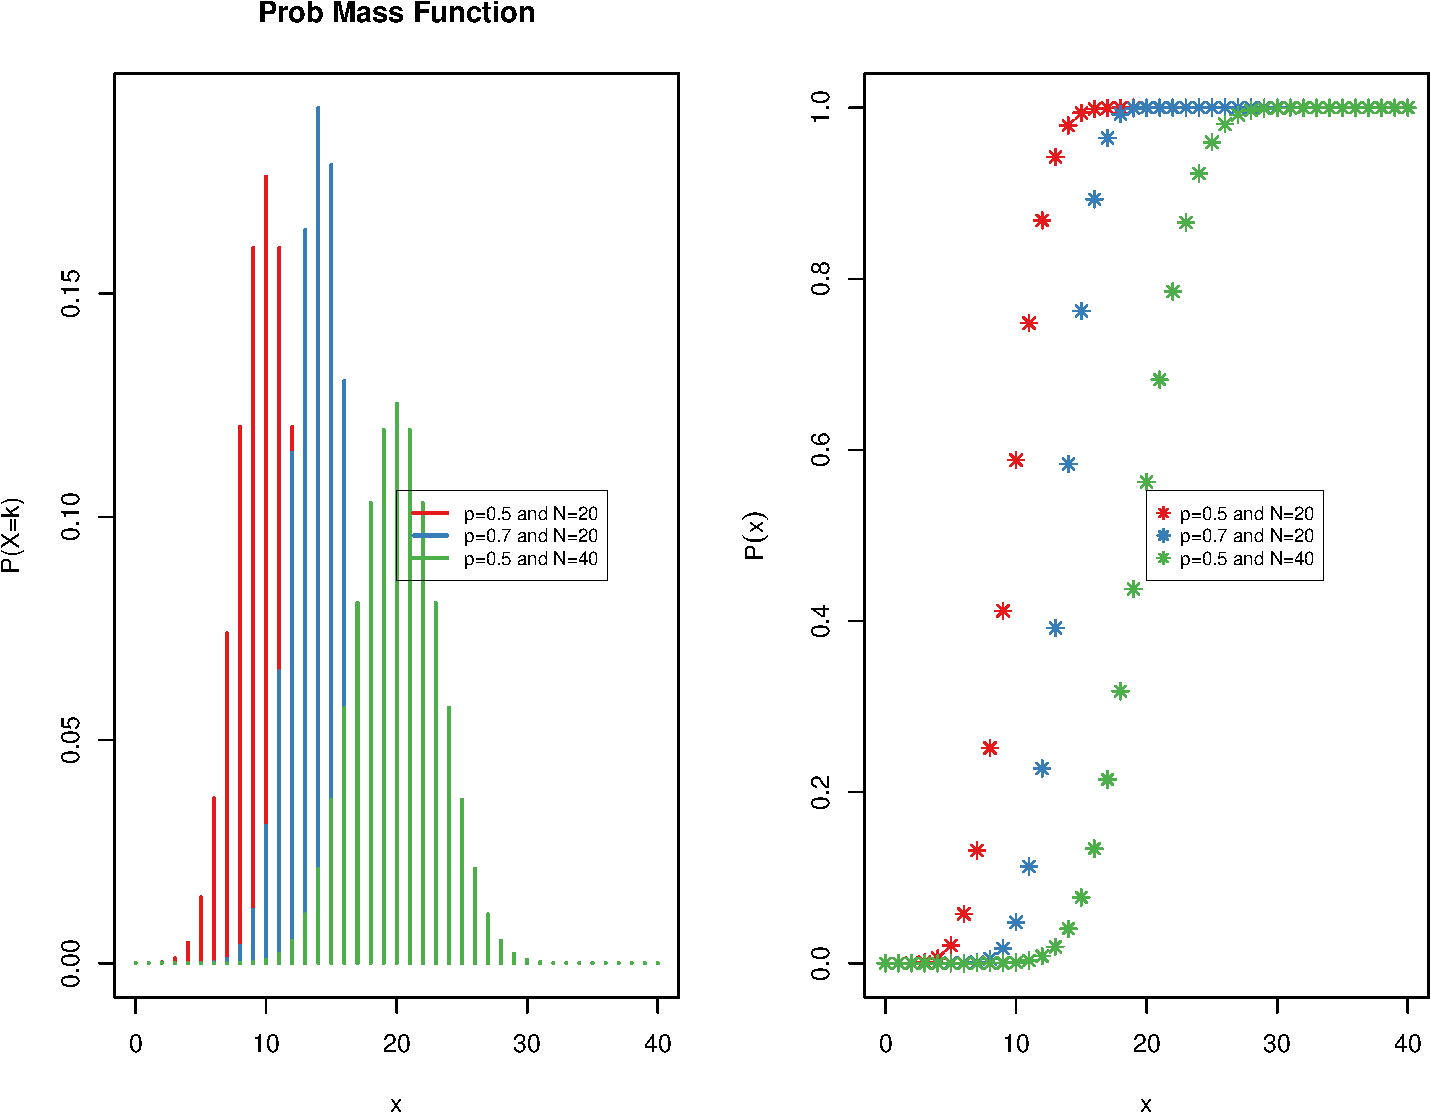
\includegraphics{tema4a_files/figure-latex/unnamed-chunk-1-1.pdf}

\subsection{Axiomas de probabilidad}\label{axiomas-de-probabilidad}

Dado un espacio muestral, \(E\), definimos probabilidad como una
función, \(P\), que asigna a un suceso \(A\) un valor numérico \(P(A)\),
verificando las siguientes reglas (axiomas)

\begin{enumerate}
\def\labelenumi{\arabic{enumi}.}
\item
  \(0\leq P(A) \leq 1\)
\item
  \(P(E)=1\)
\item
  \(P(A\cup B)=P(A)+P(B)\) si \(A\in B = \emptyset\)
\end{enumerate}

El tercer axioma se generaliza a cualquier número de sucesos de
disjuntos:

\includegraphics[width=0.75000\textwidth]{pics/union.png}

y por tanto

\[
  Pr\left( \cup_{i=1}^{5}A_i\right) = \sum_{i}^5 Pr(A_i)
 \]

Estos axiomas no asignan probabilidades a sucesos, pero facilitan el
cálculo de probabilidades de unos sucesos a partir de la probabilidad de
otros:

\begin{enumerate}
\def\labelenumi{\arabic{enumi}.}
\item
  \(Pr(\bar{A}) = 1-Pr(A) \rightarrow E = A \cup \bar{A} \rightarrow Pr(A) + Pr(\bar{A})\)
\item
  \(Pr(\emptyset) = 0\) \(\rightarrow \emptyset = E\)
\item
  Si \(A \subseteq B \rightarrow P(A) \leq P(B)\)
\end{enumerate}

\subsection{Teorema de Bayes}\label{teorema-de-bayes}

Si \(A_1, A_2 ,... , A_n\) son:

\begin{itemize}
\item
  Sucesos incompatibles 2 a 2.
\item
  Cuya unión es el espacio muestral
  (\(A_1 \cup A_2 \cup... \cup A_n = E\)).
\item
  Y \(B\) es otro suceso.
\end{itemize}

El teorema de Bayes nos dice que:

\[
P(A_i|B)  = \frac{P(A_i) \cdot P(B|A_i)}{P(B)}
\]

donde \[
 P(B) = P(A_1) \cdot P(B|A_1) + P(A_2) \cdot P(B|A_2) + ... +P(A_n) \cdot P(B|A_n)
\]

Las probabilidades \(p(A_i)\) se denominan probabilidades a priori.

Las probabilidades \(p(A_i/B)\) se denominan probabilidades a
posteriori.

Las probabilidades \(p(B/A_i)\) se denominan verosimilitudes.

\medskip

\textbf{Ejemplo 1} El 20\% de los empleados de una empresa son
ingenieros y otro 20\% son economistas. El 75\% de los ingenieros ocupan
un puesto directivo y el 50\% de los economistas también, mientras que
los no ingenieros y los no economistas solamente el 20\% ocupa un puesto
directivo. ¿Cuál es la probabilidad de que un empleado directivo elegido
al azar sea ingeniero?

\emph{Solucion}

¿\(P(Ingeniero|Directivo)\)?

\includegraphics[width=0.60000\textwidth]{pics/bayes1.png}

\begin{eqnarray*}
P(Ingeniero|Directivo) & = & \frac{P(Ingeniero) \times P(Directivo|Ingeniero)}{P(Directivo)} = \\ 
& = & \frac{0.2\times 0.75}{0.2 \times 0.75 + 0.2 \times 0.5 + 0.6 \times 0.2} = 0.405
\end{eqnarray*}

\textbf{Ejemplo 2}

La probabilidad de que haya un accidente en una fábrica que dispone de
alarma es 0.1. La probabilidad de que suene esta sí se ha producido
algún incidente es de 0.97 y la probabilidad de que suene si no ha
sucedido ningún incidente es 0.02.

En el supuesto de que haya funcionado la alarma, ¿cuál es la
probabilidad de que no haya habido ningún incidente?

\emph{Solucion}

Sean los sucesos:

\(I = \mbox{`Producirse incidente'}\).

\(A = \mbox{`Sonar la alarma'}\).

\includegraphics[width=0.60000\textwidth]{pics/bayes2.png}

\(P(\bar{I}|A) = \frac{P(\bar{I}) \times P(A|\bar{I})}{P(A)} = \frac{0,9\times 0,03}{0,1\times 0,97 + 0,9 \times 0,02}=0,157\)

\end{document}